\documentclass{article}

\textwidth=6.5in
\textheight=8.5in
\voffset=-54pt
\oddsidemargin=0in
\evensidemargin=0in
\setlength{\parskip}{8pt}
\setlength{\parindent}{0pt}

\usepackage{amsmath, amssymb}
\usepackage{ifthen}

\usepackage[inline]{enumitem}
\setlist{topsep=0pt, parsep=8pt}

\usepackage[rgb,table]{xcolor}\convertcolorsUfalse
\usepackage{graphicx}

% change hyperref options
\PassOptionsToPackage{hyphens}{url}
\usepackage[bookmarks,colorlinks,linkcolor=black,citecolor=blue,pdfstartview=FitH,urlcolor=blue]{hyperref}
\hypersetup{pdfpagemode=UseNone}
\usepackage{bookmark}

\usepackage{graphicx}
\usepackage{multicol}
\usepackage{framed}
\usepackage{array}

\usepackage{icomma}

\usepackage{soul}

\usepackage{pgfplots}
\pgfplotsset{compat=1.18}  
\pgfplotscreateplotcyclelist{mycolor}{black, blue, red, green!70!black, magenta, purple, cyan, orange }  
\pgfplotsset{
  disabledatascaling,
  cycle list=tikzcolor, 
  axis lines=middle,
  every axis plot/.style={no marks, thick},
  every axis/.style={
    enlarge x limits=false,
    enlarge y limits=auto,
    xlabel style={at={(current axis.right of origin)},anchor=west},
    ylabel style={at={(current axis.above origin)},anchor=south},
    % extra x and y ticks for asymptotes
    extra x tick style={grid=major, grid style={dashed,black}},
    extra y tick style={grid=major, grid style={dashed,black}},
    /pgf/number format/1000 sep={},
  },    
  tick label style = {font=\footnotesize, fill=\currentbgcolor, inner sep=0pt},    
  xticklabel shift=1pt,    
  scaled ticks=false,
  scaled y ticks=false,
  unbounded coords=jump,
  samples=101,
  minor tick length=0,
  scatter/classes={
    open={mark=*,draw=black,fill=white, mark size=2, thin},
    closed={mark=*,draw=black,fill=black, mark size=2, thin}
  },
  width=3in,
}
\pgfplotsset{open/.style={only marks, mark=*, fill=white, thin, mark size=2}}
\pgfplotsset{closed/.style={only marks, mark=*, draw=black, fill=black,
    thin, mark size=2}}
\pgfplotsset{labeled/.style={nodes near coords, only marks, mark=*, draw=black, fill=black, thin, mark size=2, point meta=explicit symbolic}}

\usepackage{tikz}
\usetikzlibrary{
  matrix,%
  % enables the snake paths
  decorations.pathmorphing,%
  % enables bigger arrows
  decorations.markings,%
  decorations.pathreplacing,%
  decorations.text,%
  calc,%
  patterns,%
  shapes.geometric,%
  arrows,
  decorations.shapes,
  positioning,
  plotmarks,
  intersections
}
\tikzset{>=latex} % sets default arrow type in tikz
\tikzset{font=\normalsize}
\tikzset{mark size=1.5pt, mark options=thin}
\tikzset{pin distance=4pt,
  every pin edge/.style={<-, thin, shorten <= -2pt}}

\interfootnotelinepenalty=10000
\renewcommand{\thefootnote}{(\arabic{footnote})}

\usepackage{multirow, bigdelim}

% change to \usepackage[sols]{handout} to see solutions
\usepackage[sols]{handout}
\renewcommand{\workshopnote}{CA Notes.}    

\newcommand\iscurrentenumi[1]{%
  \ifthenelse{\equal{#1}{\theenumi}}{}{#1}}
\setenumerate[1]{ref=\#\arabic*}
\setenumerate[2]{ref=\protect\iscurrentenumi{\theenumi}(\alph*)}
\newcommand\enumiiprefix[2]{%
  \ifthenelse{{\equal{#1}{\theenumi}}\AND{\equal{#2}{(\alph{enumii})}}}{}{}%
  \ifthenelse{{\equal{#1}{\theenumi}}\AND{\NOT{\equal{#2}{(\alph{enumii})}}}}{#2}{}%
  \ifthenelse{\equal{#1}{\theenumi}}{}{#1#2}%
}
\setenumerate[3]{ref=\protect\enumiiprefix{\theenumi}{(\alph{enumii})}\roman*}

\definecolor{purple}{rgb}{0.5,0,1.0}

\definecolor{magenta}{rgb}{1, 0, 0.5}

\definecolor{skyblue}{rgb}{0, 0.5, 1}

\usepackage{fancyhdr}
\lhead{\textcolor{white}{This content is protected and may not be shared, uploaded, or distributed.}}
\rhead{}
\rfoot{\vspace*{\fill}\footnotesize\textcopyright{} \emph{Harvard Math Ma}}
\renewcommand{\headrulewidth}{0pt}
\pagestyle{fancy}
\begin{document}

\htitle{Workshop 2}

\begin{workshop}
  Throughout the semester, we'll be using workshop time to introduce students to metacognitive learning strategies. Here's a nice quote from \emph{Teach Yourself How to Learn} by Saundra Yancy McGuire (she's an expert on teaching and learning): ``\emph{Metacognition}, a term coined by John H. Flavell (1976), is \emph{thinking about your own thinking}\ldots When you use metacognition, you become consciously aware of yourself as a problem solver, which enables you to actively seek solutions to any problems you may encounter, rather than relying on others to tell you what to do or to answer your questions. As you make the transition from being a passive student to being a proactive learner, you will gain the ability to monitor, plan, and control your mental processing. In other words, instead of staggering through a maze, using instinct alone to look for cheese, you will become aware that you need to plot a course and search systematically for cheese, keeping track of what works and what doesn’t. Metacognition also gives you the ability to accurately judge how deeply you have learned something, whether you have only a superficial understanding or the ability to widely apply your knowledge. For example, while studying, you might start to ask yourself, “Am I understanding this material, or just memorizing it?” When you use metacognition, you become tremendously empowered as a learner because you begin to be able to teach yourself.''

  Today, we'll have students do a mini-exam inventory, where they practice assessing their own understanding. This is in a Google Doc in the workshops folder. 

  \begin{center}
    \rule{5in}{0.4pt}
  \end{center}

  The first two problems today are review of topics that the mini-exam will cover. \ref{income-tax} is practice with piecewise linear functions and  illustrates how these show up in the world, so it's worth having students spend the time to really understand this one.
\end{workshop}

\begin{enumerate}
\item 

  \begin{enumerate}
  \item
    \begin{problem}[\vfill]
      On a single set of axes, graph $f(x) = 1 - \sqrt{x + 2}$ in one color and $g(x) = -2x$ in another.
    \end{problem}

    \begin{solution}

    \begin{tikzpicture} 
        \begin{axis}[xmax=4, ymax=2, ymin=-2, width=4in, height=3in]
          \addplot+[domain=-4:4, skyblue]{1-(x+2)^.5};
          \addplot+[domain=-4:4, magenta]{-2*x};
        \end{axis}
      \end{tikzpicture}
      \end{solution}

  \item

    \begin{workshop}
      If students are puzzled by the extraneous solutions bit, you can help them understand that squaring an equation can introduce additional solutions. For example, if I square both sides of $x = \sqrt{5}$, I get $x^2 = 5$, but this actually has two solutions $x = \pm \sqrt{5}$.
    \end{workshop}

    \begin{problem}[\vfill]
      At how many points do the graphs of $f$ and $g$ intersect? Find the coordinates of each point of intersection.

      (\emph{Note:} When you solve an equation involving a square root, you often end up with extraneous solutions. So, you should plug each possible solution back into the original equation to check whether it actually works.)
    \end{problem}

    \begin{solution}
    We want to know where $f(x)=g(x)$.
\begin{align*}
    1-\sqrt{x+2}&=-2x\\
    1+2x&=\sqrt{x+2}\\
    (1+2x)^2&=(\sqrt{x+2})^2\\
    1+4x+4x^2&=x+2\\
    4x^2+3x+-1&=0    
\end{align*}
Applying the quadratic formula to find the zeros of the equation, we have:
\begin{align*}
    x&= \frac{-3\pm\sqrt{3^2-4(4)(-1)}}{2(4)}\\
x&=\frac{-3\pm\sqrt{25}}{8}\\
x&=\frac{-3\pm 5}{8}=\frac{1}{4},\, -1\\
\end{align*}
Checking these solutions, we find $f(-1) \neq g(-1)$, but $f(\frac{1}{4})=g(\frac{1}{4})$. We've found one point of intersection when $x=\frac{1}{4}$. We can find the y-value by evaluating either equation. $2(\frac{1}{4})=\frac{1}{2}$. The coordinates of the point are $\displaystyle\bigg( \frac{1}{4}, \frac{-1}{2}\bigg)$.
    \end{solution}
  \end{enumerate}

\item 
  \begin{problem}[\nstretch{0.4}]
    Simplify $\left( \sqrt[3]{x} \cdot x^{1/6} \right)^4 + 16^{-3/4}$
  \end{problem}

  \begin{solution}
  \begin{align*}
      \left( \sqrt[3]{x} \cdot x^{1/6} \right)^4 + 16^{-3/4}&= (x^{1/3}\cdot x^{1/6})^4 + (16^{1/4})^{-3}\\
      &=(x^{2/6}x^{1/6})^4+(2)^{-3}\\
      &=(x^{1/2})^4+\frac{1}{2^3}\\
      &=x^2+\frac{1}{8}
      \end{align*}
  \end{solution}

\item  \label{income-tax}

  \begin{workshop}
    This is really how the U.S. income tax system works!
  \end{workshop}

  \begin{enumerate}
  \item
    \begin{problem}[\stretch{1.2}]
      For the 2023 tax year, here's how the U.S. income tax system works for single taxpayers who make under \$95,000 in taxable income. They pay 10\% on taxable income below \$11,000, 12\% on taxable income between \$11,000 and \$44,725, and 22\% on taxable income above \$44,725. Write a function $T(M)$ giving the number of dollars in tax a single taxpayer with \$$M$ of taxable income owes (for $0 \leq M \leq 95,000$), and sketch the graph of $T(M)$.
    \end{problem}

    \begin{solution}
      A person whose income $M$ is $\leq 11,000$ pays 10\% of their income, which is exactly $0.1 M$. So, $T(M) = 0.1 M$ when $M \leq 11,000$.

      A person whose income $M$ is between $11,000$ and $44,725$ pays \[ \underbrace{\text{10\% tax on the first \$11,000 of income}}_{0.1 (\$11,000) = \$1100} {}+{} \underbrace{\text{12\% on taxable income above \$11,000}}_{0.12 (M - 11,000)}.\] Thus, such a person pays a total of $1100 + 0.12 (M - 11,000)$.

      Finally, a person with income $M$ over $\$44,725$ pays
      \[ \underbrace{\text{10\% on first \$11,000}}_{0.1 (\$11,000) = \$1100} {}+{} \underbrace{\text{12\% on income between \$11,000 and \$44,725}}_{0.12 (\$44,725 - \$11,000) = \$4047} {}+{} \underbrace{\text{22\% on income above \$44,725}}_{0.22 (M - 44,725)}, \] for a total of $5147 + 0.22 (M - 44,725)$.

      So, $\boxed{T(M) =
        \begin{cases}
          0.1 M & \text{ if } M \leq 11,000 \\
          1100 + 0.12 (M - 11,000) & \text{ if } 11,000 < M \leq 44,725 \\
          5147 + 0.22 (M - 44,725) & \text{ if } 44,725 < M
        \end{cases}}$.

      Here is the graph of this function:
      \begin{center}
        \begin{tikzpicture}
          \begin{axis}[disabledatascaling=false, xtick={11000, 44725, 95000}, width=4in, height=3in, ytick={1100, 5147}, xlabel={taxable income}, ylabel={tax}, enlarge x limits=auto]
            \addplot+[domain=0:11000, skyblue]{0.1*x}; \addplot+[domain=11000:44725, magenta]{1100 + 0.12*(x-11000)}; \addplot+[domain=44725:95000, green!80!black]{5147 + 0.22 * (x-44725)};
          \end{axis}
        \end{tikzpicture}
      \end{center}
      The blue piece has slope $0.1$, the pink piece has slope $0.12$, and the green piece has slope $0.22$.
    \end{solution}

  \item

    \begin{workshop}
      This is a very common misconception, and it would be great for students to come away with the understanding that this is absolutely not true! 
    \end{workshop}

    \begin{problem}[\stretch{0.75}]
      Your friend currently has a yearly taxable income of \$40,000. Their boss offers them a \$5000 raise, but your friend says, ``I don't want it! That will put me in the 22\% tax bracket, so I'll pay more taxes and end up taking less money home.'' Assess your friend's argument.
    \end{problem}

    \begin{solution}
        Calculating $T(40000)$, we have $T(40000)=1100+0.12(40000-11000)=1100+3480=4580$, takehome pay is $40000-4580=\$34420$\\
        Calculating $T(45000)$, we have $T(45000)=5147+0.22(45000-44725)=5147+60.5=\$5207.50$, so takehome pay will be $45000-5207.50=\$39792.50$\\
        While your friend will have to pay more in taxes, their raise more than makes up for it and they end up taking more money home.
    \end{solution}

  \item

    \begin{workshop}
      This is another way to emphasize that being in the 22\% tax bracket doesn't mean paying 22\% on all taxable income.
    \end{workshop}

    \begin{problem}[\stretch{0.3}]
      If your friend takes the \$5000 raise, what percent of their total taxable income will they pay in taxes? (This is called their ``effective tax rate''.)
    \end{problem}

    \begin{solution}
        $\frac{5207.50}{45000}=.1157\hdots\approx 11.6\%$
    \end{solution}
    
  \item
    \begin{problem}[\stretch{0.8}]
      Graph the ``slope function'' $T'(M)$, which gives the slope at every
      point on the graph of $T(M)$. 
    \end{problem}

    \begin{solution}
         \begin{tikzpicture} 
        \begin{axis}[disabledatascaling=false, xtick={11000, 44725, 95000}, width=4in, height=3in, ytick={0.1, 0.12, 0.22}, xlabel={taxable income}, ylabel={tax}, enlarge x limits=auto]
          \addplot+[domain=0:11000, skyblue] {0.1};
          \addplot+[domain=11000:44725, magenta] {0.12};
          \addplot+[domain=44725:95000, green] {0.22};
          \addplot[open] coordinates{(0, 0.1)(11000, 0.1)(11000, .12) (44725, .12) (44725, .22)};
        \end{axis}
      \end{tikzpicture}
    \end{solution}

  \item
    \begin{problem}[\nstretch{0.2}]
      What's the practical meaning of $T'(M)$? 
    \end{problem}

    \begin{solution}
        $T'(M)$ tells us the rate at which the amount of tax paid is changing per additional dollar of income. For example, someone with \$30,000 taxable income, tax is increasing at a rate of \$0.12 per additional dollar of taxable income.
    \end{solution}
  \end{enumerate}

\item 
  \begin{problem}[\newpage]
    You're designing a box with no top for raspberry picking. The base is a square with sides of length $s$ and the volume is $250$ in$^3$. The material for the base costs $3$ cents per square inch and the sides cost $2$ cents per square inch.

    Write a function $C(s)$ that gives the cost of the material (in cents)
    used in making the box as a function of $s$, the length of the side of
    the base.  What is the domain of your function?
  \end{problem}

  \begin{solution}
    We're trying to find the cost of the box; since the box is made out
    of two different materials, we can first break the cost down as
    \begin{align*}
      \text{cost of box} &= \text{cost of sides} + \text{cost of base} \\
      \intertext{We are given the cost per unit area for each type of
        material.}
      &= (\text{cost per unit area of sides})(\text{area of sides}) +
      (\text{cost per unit area of base})(\text{area of base}) \\
      &= 2 (\text{area of sides}) + 3 (\text{area of base}) \\
      \intertext{The area of the base is $s^2$.  To describe the area of
        the sides, it would helpful to have a variable for the height of
        the box; let's call that $h$.  There are 4 sides, each $s$ inches
        wide and $h$ inches tall, for a total area of $4sh$:}
      &= 2 (4 sh) + 3s^2\\
      &= 8sh + 3s^2 \\
      \intertext{Finally, we need to express $h$ in terms of $s$ to get
        everything in terms of $s$.  We are told that the volume of the
        box is $250$, so $s^2 h = 250$.  Therefore, $h =
        \frac{250}{s^2}$.}
      &= 8 s \cdot \frac{250}{s^2} + 3s^2 \\
      &= \boxed{\frac{2000}{s} + 3s^2}
    \end{align*}
  \end{solution}

\item  \label{gottlieb-1.2.11} % 1.2.11

  Let $C$ be a circle of radius $1$ and let $A(n)$ be the area of a regular $n$-gon inscribed in the circle. For instance, $A(3)$ is the area of an equilateral triangle inscribed in circle $C$, $A(4)$ is the area of a square inscribed in circle $C$, and $A(5)$ is the area of a regular pentagon inscribed in circle $C$. (A polygon inscribed in a circle has all its vertices lying on the circle. A regular polygon is a polygon whose sides are all of equal length and whose angles are all of equal measure.)

  \begin{enumerate}
  \item
    \begin{problem}[\vfill]
      Find $A(4)$.
    \end{problem}   

    \begin{solution} 
      A ``regular 4-gon'' is a square. The following picture is useful in finding the area of a square that can be inscribed in a circle of radius 1.
      \begin{center} 
        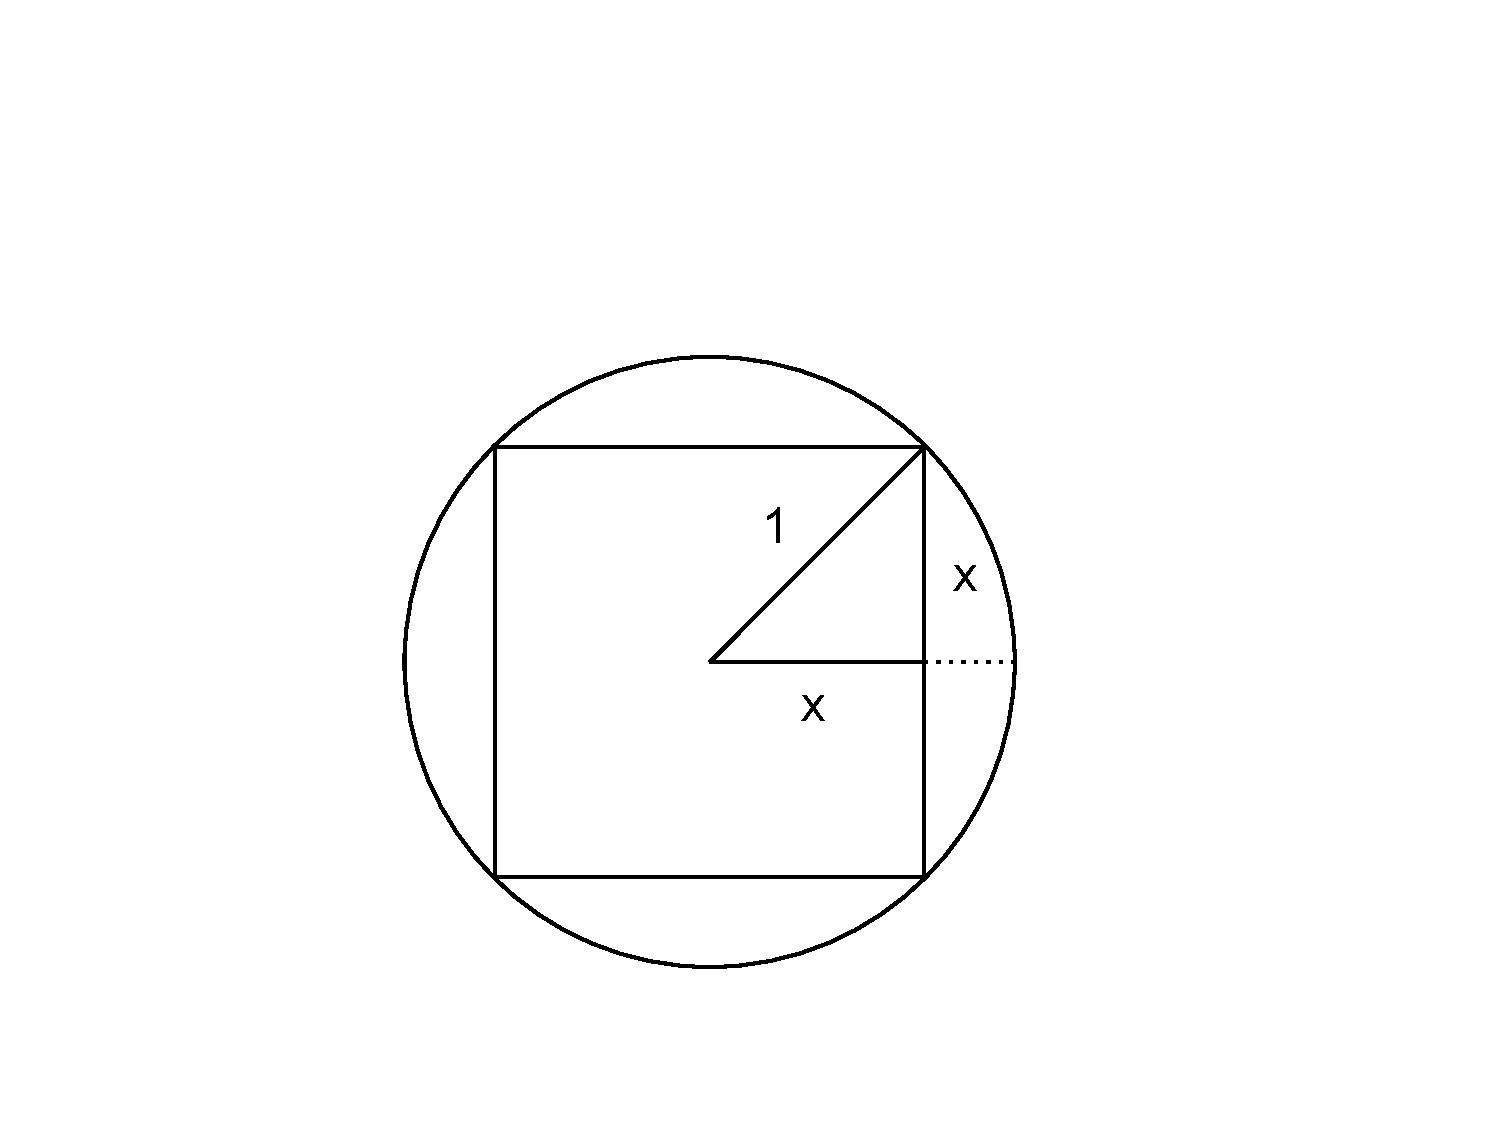
\includegraphics[width=2in]{images/circlesquare.pdf}
      \end{center} 

      Each side of the square has length $2x$, so the area of the square is $(2x)^2$.  By the Pythagorean Theorem, $x^2 + x^2 = 1^2$, i.e. $x=\sqrt{1/2}$.  So $A(4)$, the area of the square is $(2\sqrt{1/2})^2 = 2$.

    \end{solution} 

  \item
    \begin{problem}[\vfill]
      What is the domain of $A(n)$?
    \end{problem}

    \begin{solution} 

      The largest domain for $A(n)$ is the set of all integers greater than or equal to 3, since a polygon can have any integer greater than three number of sides.  A ``$2$-gon" doesn't make sense, nor does a ``$-3$-gon or a``$2.7$" gon.

    \end{solution}

  \item
    \begin{problem}[\vfill]
      As $n$ increases, do you think that $A(n)$ increases or decreases? This is hard to justify rigorously, but what does your intuition tell you?
    \end{problem}

    \begin{solution} 
      As $n$ increases, $A(n)$ should also increase.  One way to see this is that as $n$ increases, the $n$-gons {\it look} more and more like the circle.  There is less and less space lost between the edges of the $n$-gon the circle outside.  This is illustrated in the following picture:\footnote{ from \url{http://www.math.rutgers.edu/~erowland/polygons-project.html}}

      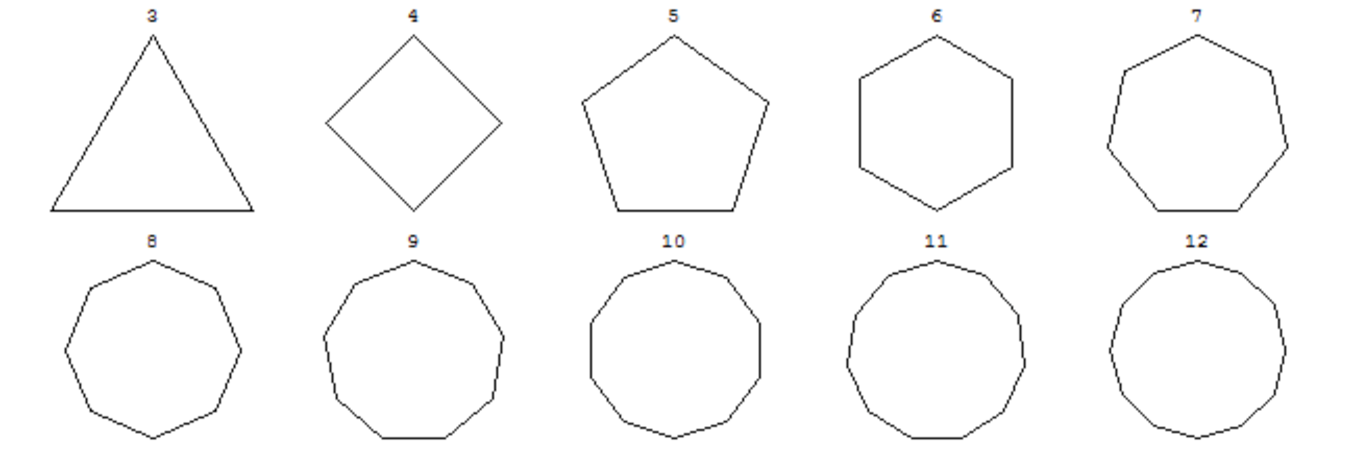
\includegraphics[width=5in]{images/polygons.pdf}

    \end{solution}

  \item
    \begin{problem}[\vfill]
      If you think $A(n)$ increases, will it increase without bound, or is there an upper bound for $A(n)$?

      If you think $A(n)$ decreases, will it decrease without bound, or is there a lower bound for $A(n)$?
    \end{problem}

    \begin{solution}       
      There is a bound on $A(n)$; it will never exceed $\pi$, since each $n$-gon must fit inside the circle of radius 1, whose area is $\pi$
    \end{solution}

  \end{enumerate}

\end{enumerate}
\end{document}
